\documentclass[10pt, a4paper, twosize]{article}
%\documentclass[12pt, a4paper, twoside]{book}

\usepackage{helvet}
\usepackage{hyperref}
\usepackage{graphicx}
\usepackage{listings}
\usepackage{textcomp}
\usepackage[
	a4paper,
	outer=2cm,
	inner=4cm,
	top=2cm,
	bottom=2cm
]{geometry}
\usepackage{float}
\usepackage{tabularx}
\usepackage[disable]{todonotes}
\usepackage{color, soul}
\usepackage{amsmath}
\usepackage{algorithmicx}
\usepackage[noend]{algpseudocode}
\usepackage{algorithm}
\usepackage{framed}
\usepackage{subcaption}
\usepackage{titlepic}
\usepackage{fancyhdr}
\usepackage[simplified]{styles/pgf-umlcd}
\usepackage{shorttoc}
\usepackage{url}
\usepackage{paralist}

\definecolor{grey}{rgb}{0.9, 0.9, 0.9}
\definecolor{dkgreen}{rgb}{0,0.6,0}
\definecolor{dkred}{rgb}{0.6,0,0.0}

\lstdefinestyle{DOS}
{
    backgroundcolor=\color{black},
    basicstyle=\scriptsize\color{white}\ttfamily,
    stringstyle=\color{white},
    keywords={}
}

\lstdefinestyle{makefile}
{
    numberblanklines=false,
    language=make,
    tabsize=4,
    keywordstyle=\color{red},
    identifierstyle= %plain identifiers for make
}

\lstset{
  language=Java,                % the language of the code
  basicstyle=\footnotesize\ttfamily,
  numbers=left,                   % where to put the line-numbers
  stepnumber=1,                   % the step between two line-numbers. If it's 1, each line
  numbersep=5pt,                  % how far the line-numbers are from the code
  backgroundcolor=\color{white},      % choose the background color. You must add \usepackage{color}
  showspaces=false,               % show spaces adding particular underscores
  showstringspaces=false,         % underline spaces within strings
  showtabs=false,                 % show tabs within strings adding particular underscores
  frame=single,                   % adds a frame around the code
  rulecolor=\color{black},        % if not set, the frame-color may be changed on line-breaks within not-black text (e.g. comments (green here))
  tabsize=2,                      % sets default tabsize to 2 spaces
  captionpos=b,                   % sets the caption-position to bottom
  breaklines=true,                % sets automatic line breaking
  breakatwhitespace=false,        % sets if automatic breaks should only happen at whitespace
  keywordstyle=\color{blue},          % keyword style
  commentstyle=\color{dkgreen},       % comment style
  stringstyle=\color{dkred},         % string literal style
  columns=fixed,
  extendedchars=true,
  frame=single,
}

%\renewcommand{\chaptername}{Topic}

% New definitions
\algnewcommand\algorithmicswitch{\textbf{switch}}
\algnewcommand\algorithmiccase{\textbf{case}}
\algnewcommand\algorithmicassert{\texttt{assert}}
\algnewcommand\Assert[1]{\State \algorithmicassert(#1)}%
% New "environments"
\algdef{SE}[SWITCH]{Switch}{EndSwitch}[1]{\algorithmicswitch\ #1\ \algorithmicdo}{\algorithmicend\ \algorithmicswitch}%
\algdef{SE}[CASE]{Case}{EndCase}[1]{\algorithmiccase\ #1}{\algorithmicend\ \algorithmiccase}%
\algtext*{EndSwitch}%
\algtext*{EndCase}%

\pagestyle{fancy}
\fancyhf{}
\fancyhead[RO, LE]{\small \rightmark}
\fancyfoot[RO, LE]{\small \thepage}

\begin{document}

%\frontmatter

\begin{titlepage}
\vspace*{5cm}
\begin{center}

\includegraphics[width=.5\textwidth]{images/EdNapUniLogoCMYK}~\\[1cm]

\textsc{\Large Edinburgh Napier University}\\[1.5cm]

\textsc{\LARGE \bfseries Git}\\[0.5cm]

\hrulefill \\[0.4cm]
{\huge \bfseries Getting Started \\[0.4cm] }
\hrulefill \\[1.5cm]

\begin{minipage}{0.4\textwidth}
\begin{flushleft} \large
\textbf{Dr Simon Wells} \\
\end{flushleft}
\end{minipage}

\vfill

\end{center}
\end{titlepage}

%\shorttoc{Overview}{0}

%\setcounter{tocdepth}{2}
%\cleardoublepage
%\tableofcontents
%\listoffigures
%\listofalgorithms
%\addtocontents{toc}{~\hfill\textbf{Page}\par}

%\mainmatter

%\input{sections/labs/04_ui}

\section{Aims}
\paragraph{} At the end of the practical portion of this topic you will:

\begin{itemize}
\item Be able to log into the University system
\item Be able to run simple programs from the command line
\item Remember how to program simple software
\item Have retrieved some supplementary texts from an online publisher
\end{itemize}

\paragraph{} There is a lot more to Git than just what is covered in this document. You should be practising with Git, turning the add-commit-push cycle into a habit but also learning additional features as you go along. Using Git counts as a professional skill for most developers and also for the people working alongside them because it is a great collaboration tool once you know how to use it well.

\begin{framed}
{\bf{NOTICE:} Make sure to type in commands rather than copying \& pasting from this document. Whilst typing can introduce typos, copying and pasting frequently introduces errors, particularly white-space related errors, that can cause things to go awry.}
\end{framed}

\section{Getting The Software}
\paragraph{} Git on Windows is a bit different to Git on other platforms so this tutorial tries to make things similar between each platform. However there will always be slight differences. Once you have the software installed your experiences of Git should be comparable between platforms and you shold be able to directly translate your experiences from Window to Linux to OS X and back again (more or less).

\subsection{Windows}
\paragraph{} If you're on Windows go to the Git SCM website\footnote{\url{https://git-scm.com/download/win}}  - don't download the software that automatically starts downloading but instead choose the link labelled "64-bit Git for Windows Portable"\footnote{\url{https://github.com/git-for-windows/git/releases/download/v2.16.1.windows.1/PortableGit-2.16.1-64-bit.7z.exe}}. Let it download, click the exe and install it somewhere useful.

\paragraph{} When running Git you will want to click the git-bash.exe rather than git-cmd.exe. They work in different ways and the commands differ between the two. Using git-bash.exe means that we can use the same commands regardless of whether we are on a Mac, Linux, or Windows machine.

\paragraph{} When you run git-bash you will get a window that looks like a command terminal. It contains enough command line commands and Git software for you to navigate the file system, create and delete files and folders, move them around, then do all of the usual Git stuff in addition like cloning a repository or committing new files to a repository.

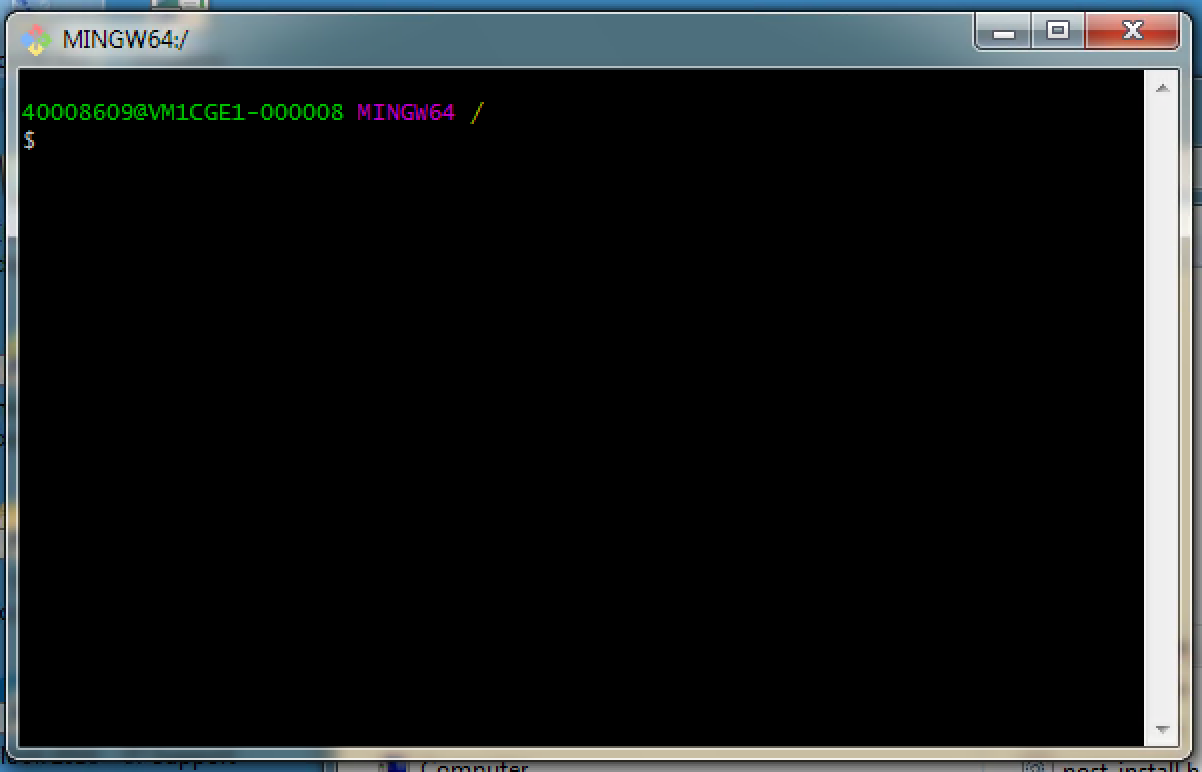
\includegraphics[width=.8\textwidth]{images/git-bash}


\subsection{MacOS}
\paragraph{} Install the Apple Command Line Developer tools (you should really have these anyway if your developing software) because one of the tools that's installed is Git:

\begin{lstlisting}
    $ xcode-select --install 
\end{lstlisting}

\paragraph{} Once the developer tools are installed you can open a terminal and type the commands that are used in the remainder of this tutorial. Note that some examples, like references to the `H:' drive aren't applicable to a Mac or Linux machine.

\subsection{Linux}
\paragraph{} Assuming a Debian based system:

\begin{lstlisting}
    $ apt-get install git
\end{lstlisting}


\section{The Most Basic Use Case for Git}

\paragraph{} We'll start by assuming that you're using a GitHub account. If not you might need to adjust some of the command a little. Start git-bash then use the following commands so that Git can label your commits with your name (obviously replacing 'Your Name' for your real world name in double quotes):

\begin{lstlisting}
    $ git config –global user.name “Your Name“
\end{lstlisting}

\paragraph{} Now tell Git which email address to associate with your commits. You should use the email address that you signed up to GitHub with:

\begin{lstlisting}
    $ git config –global user.email “example@youremail.com“
\end{lstlisting}

\paragraph{} Now, log into GitHub and create a repository. Give it a useful project name and description. 

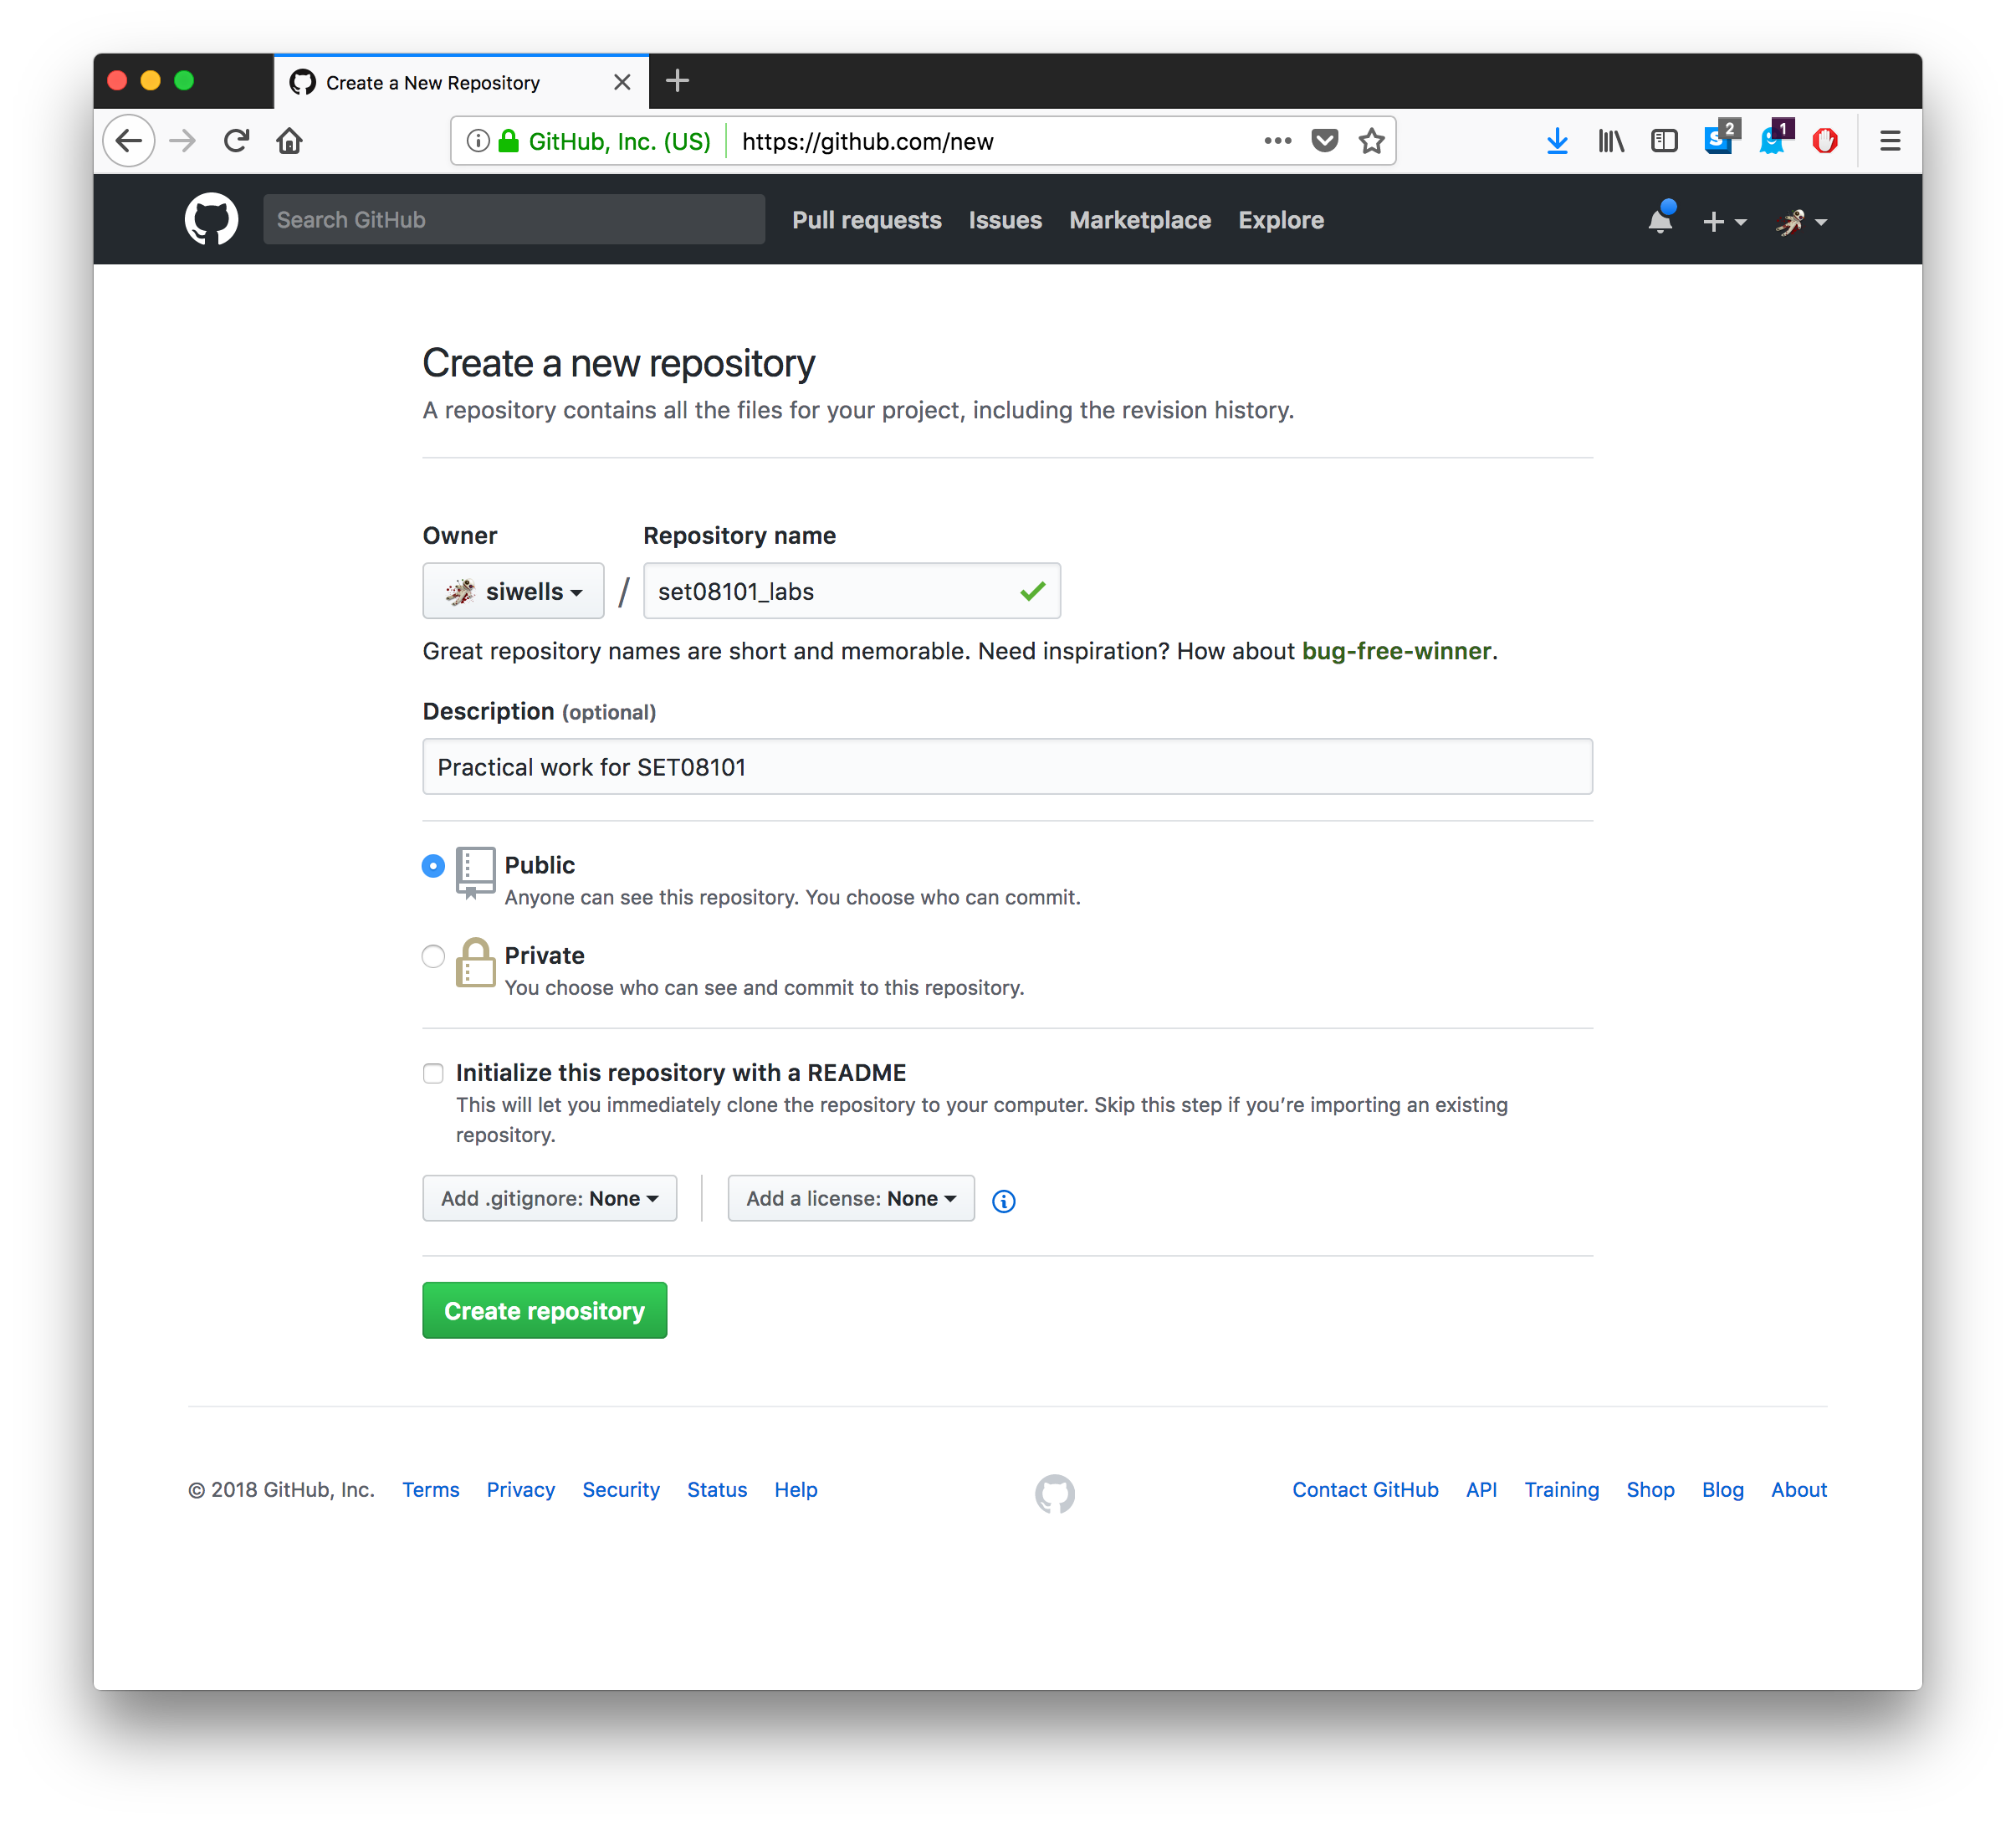
\includegraphics[width=.8\textwidth]{images/github-new-repo}

\paragraph{} Once the repository is created you will be able to clone your empty repository. This means make a copy of the repository that is on GitHub on your local machine. The address for this is available from GitHub under the green "Clone or download" button. You need to copy and paste the address, which looks something like this:

    \url{https://github.com/siwells/set08101.git}


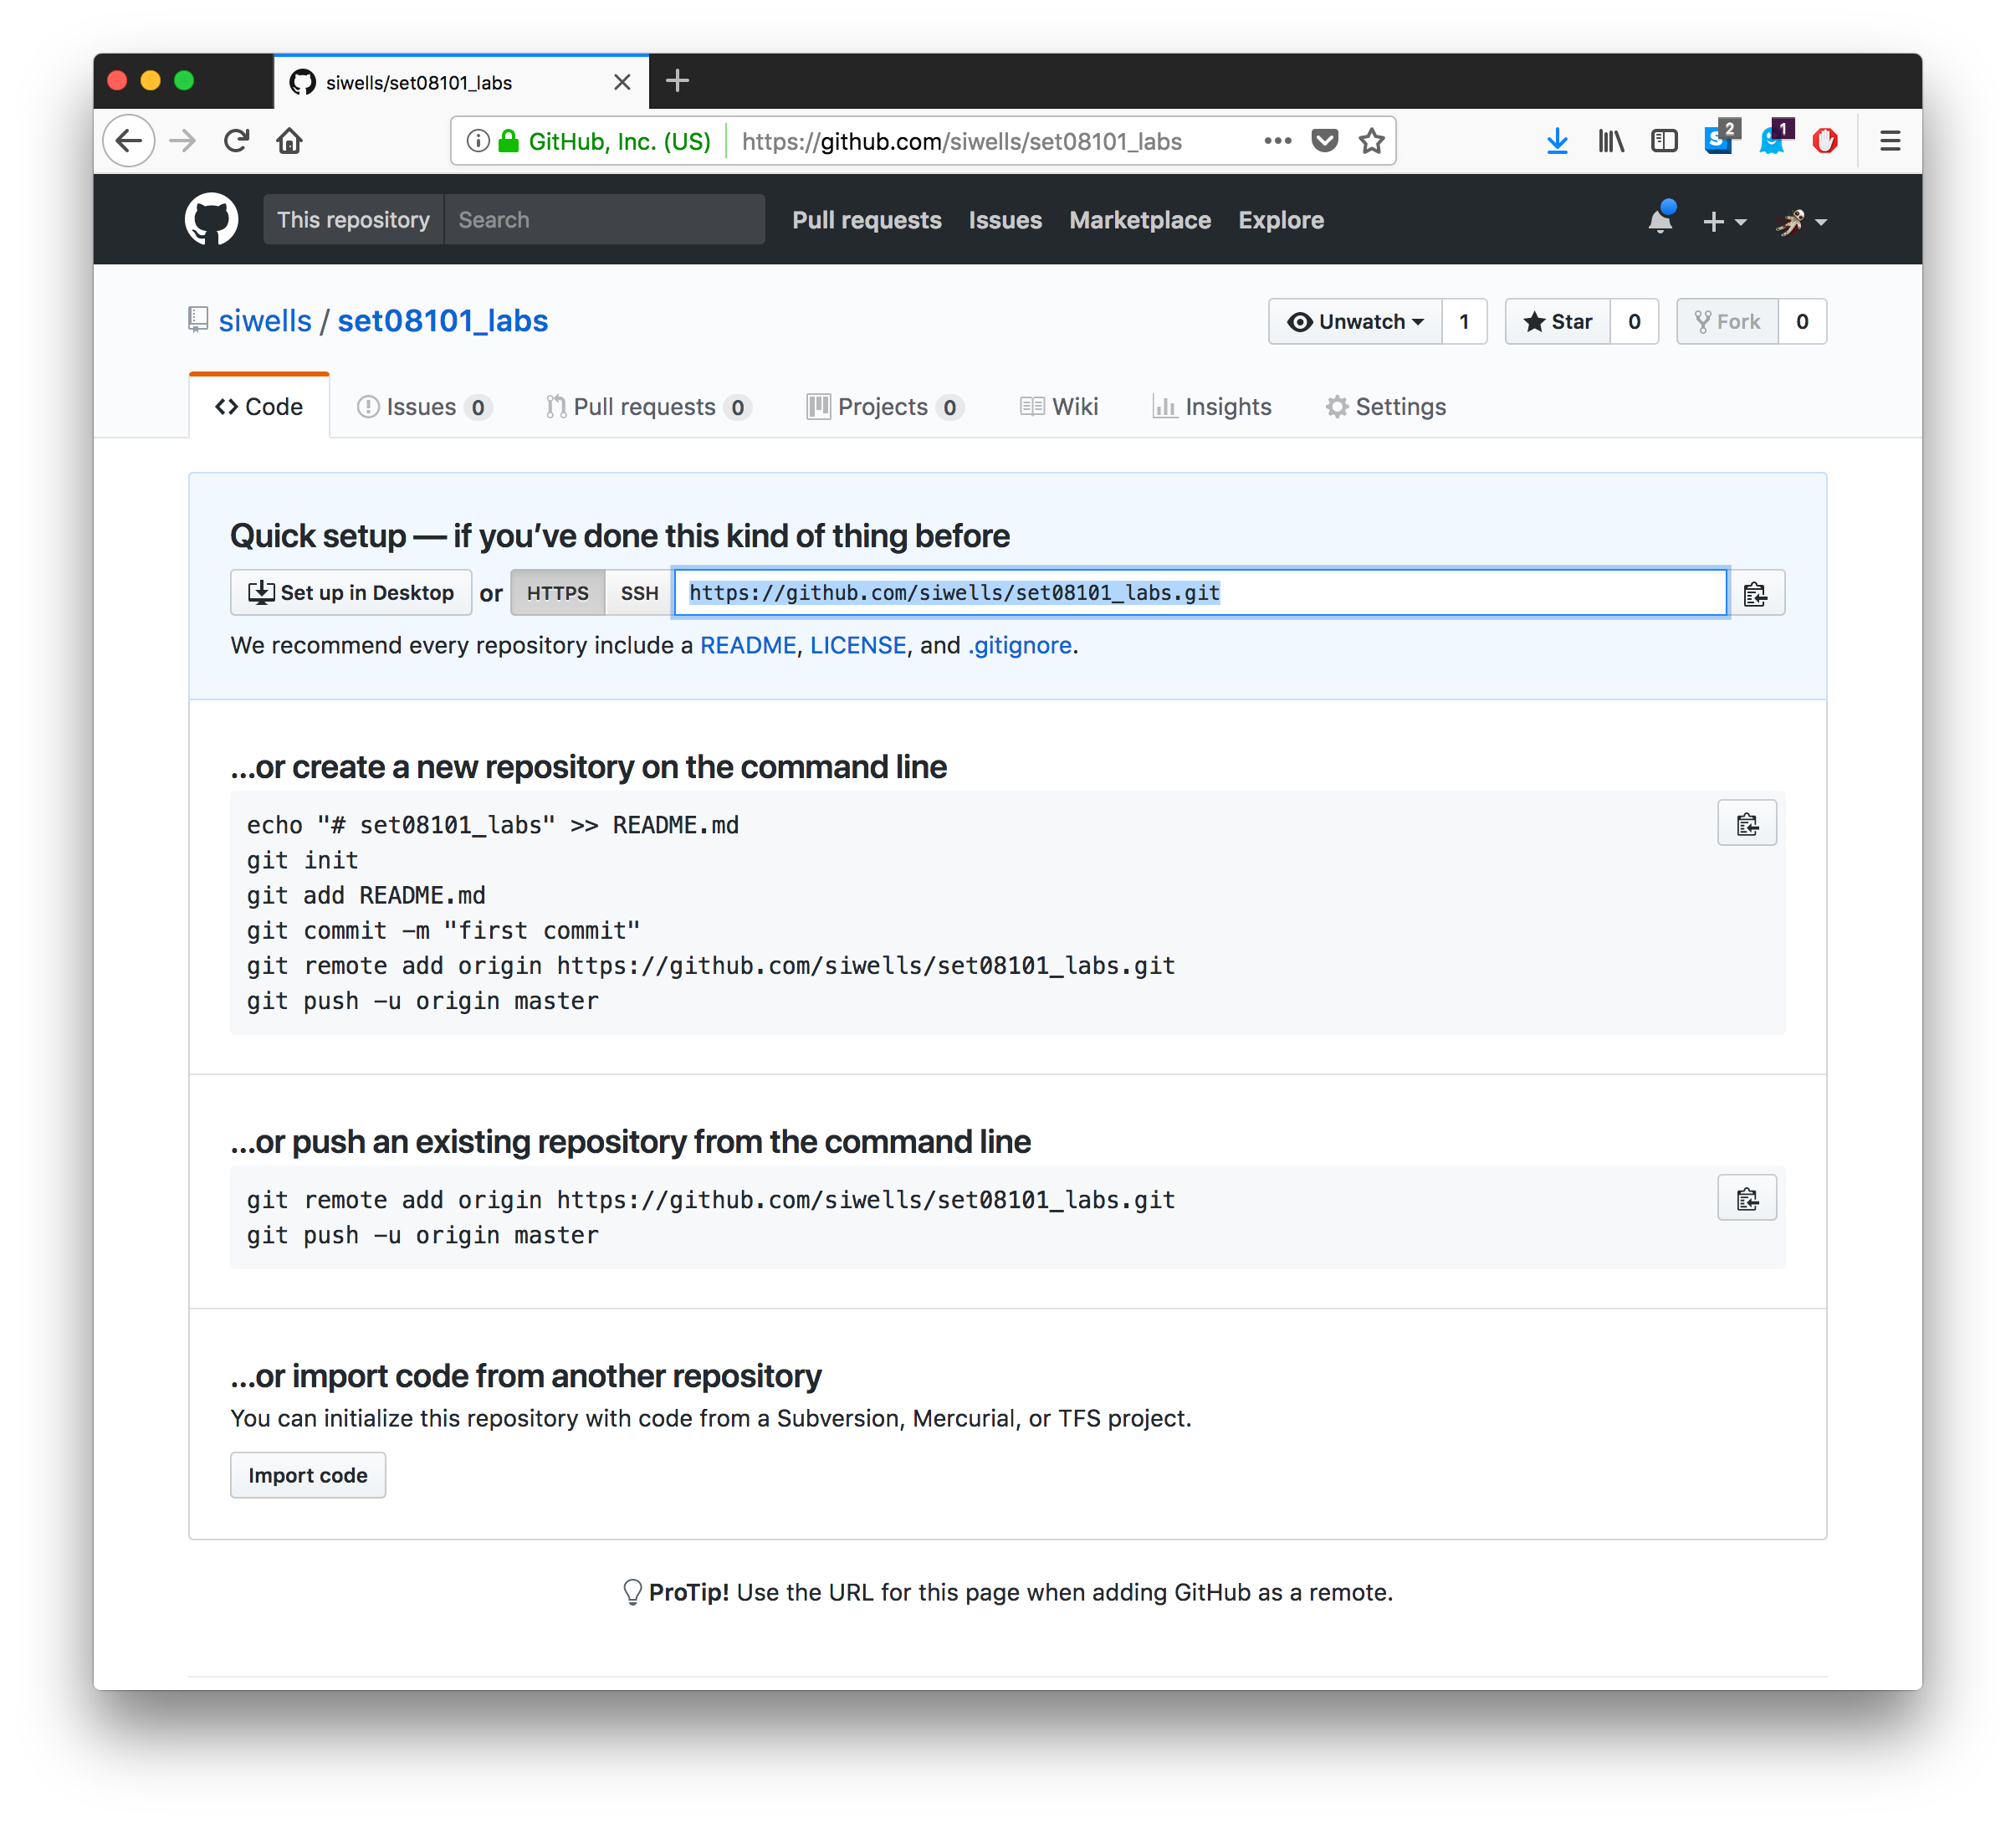
\includegraphics[width=.8\textwidth]{images/github-clone-url}

\paragraph{} so that you can use it in a command in git-bash. Note that the address contains your GitHub user name and the repository name that you used when you created the repository. You can retrieve an address that starts with either "https" or "git@github.com". For the moment we should use the one starting with "https".

\paragraph{} In your GitBash terminal you should navigate to a place on your machine where you are going to store your code, e.g. on lab machines you might want to use the H: directory. I'll assume H: from now on but your should organise your work how you see fit.

\begin{lstlisting}
    $ cd h:/
    $ mkdir set08101
    $ cd set08101
\end{lstlisting}

\paragraph{} These three commands changed the directory we were in (cd is short for change directory) then made a new directory in the new location (mkdir is short for make directory). Finally we changed directory again to move into the new set08101 directory.

\paragraph{} Now we'll clone our repository from GitHub:

\begin{lstlisting}
    $ git clone https://github.com/siwells/set08101.git
\end{lstlisting}

\paragraph{} NB. I've used the clone address for this module's repository but your should replace the address, everythin after "git clone", with what you copied from GitHub earlier.

\paragraph{} There should be some messages on screen, and when they're done there should be a message along the following lines:
\begin{lstlisting}
    You have successfully cloned to an empty repository.
\end{lstlisting}
\paragraph{} If you now type ls you should get a list of folders and one of the folders will be named for the repository that you just cloned from GitHub. This means that there is an exact copy of your repository on GitHub and one on your local machine. You can make as many clones of a repository as you like on as many machines as you like.

\paragraph{} Now you can change directory into your project folder and run Git commands on your fresh repository:

\begin{lstlisting}
    $ cd set08101
    $ git status
\end{lstlisting}

\paragraph{} The output from the git status command will look quite cryptic at the moment but you'll get used to it and quickly discover that it is telling you really important stuff about your repository and code. You can also open this folder in Window Explorer (of finder on a Mac) to manipulate your files if you find that easier but you will always need to use the git-bash program to update your repository and access the Git commands.

\paragraph{} If we add a file, e.g. hello.html to our set08101 folder then run git status again we should get a different message to before, one telling us that the repository has changed because, well, we just added a new file, and it is Git's job to notice changes. Note that Git commands only work properly within a Git repository, that means you have to cd into a folder that is within your project that Git is tracking.

\paragraph{} Whenever we add a new file to our project, or make a change to an existing file, we will need to tell Git to take note of the changes since last time. We do that with the add command:

\begin{lstlisting}
    $ git add .
\end{lstlisting}

\paragraph{} The '.' just means add all files in the repository that are either new or changed. You can also specify individual files that you want to add if you want to alter the granularity of the changes that Git tracks. Once your changes are added then you will need to commit them, this means that Git enters the changes it noticed from the add command into a record, the history, of the repository:

\begin{lstlisting}
    $ git commit -m "a commit message"
\end{lstlisting}

"a commit message" should be replaced with a short descriptive message about the changes that are being committed this helps remind you, and inform others, of why the changes that are being committed were made, e.g. "Fix file save bug" or "add new edit widget".

\paragraph{} As we develop we will keep doing this cycle of add then commit so that each change we make to our code is tracked with a descriptive message of the change. The list of messages and changes is called the history and you can inspect this using:
    
\begin{lstlisting}
    $ git log
\end{lstlisting}

\paragraph{} However adding and committing is only tracking changes locally. If we want to make sure that there is a copy of our repository on GitHub then we need to "push" changes to GitHub. We do this with the push command:

\begin{lstlisting}
    $ git push
\end{lstlisting}

\paragraph{} You should now be able to see the changes on the repositories GitHub page (you might need to refresh it first). Note that if this hasn't worked then you can try adding the repository address to the end of the command, e.g. \$ git push https://github.com/siwells/set08101.git - although make sure to change this address for your own as you won't have permissions to update the set08101 repository.

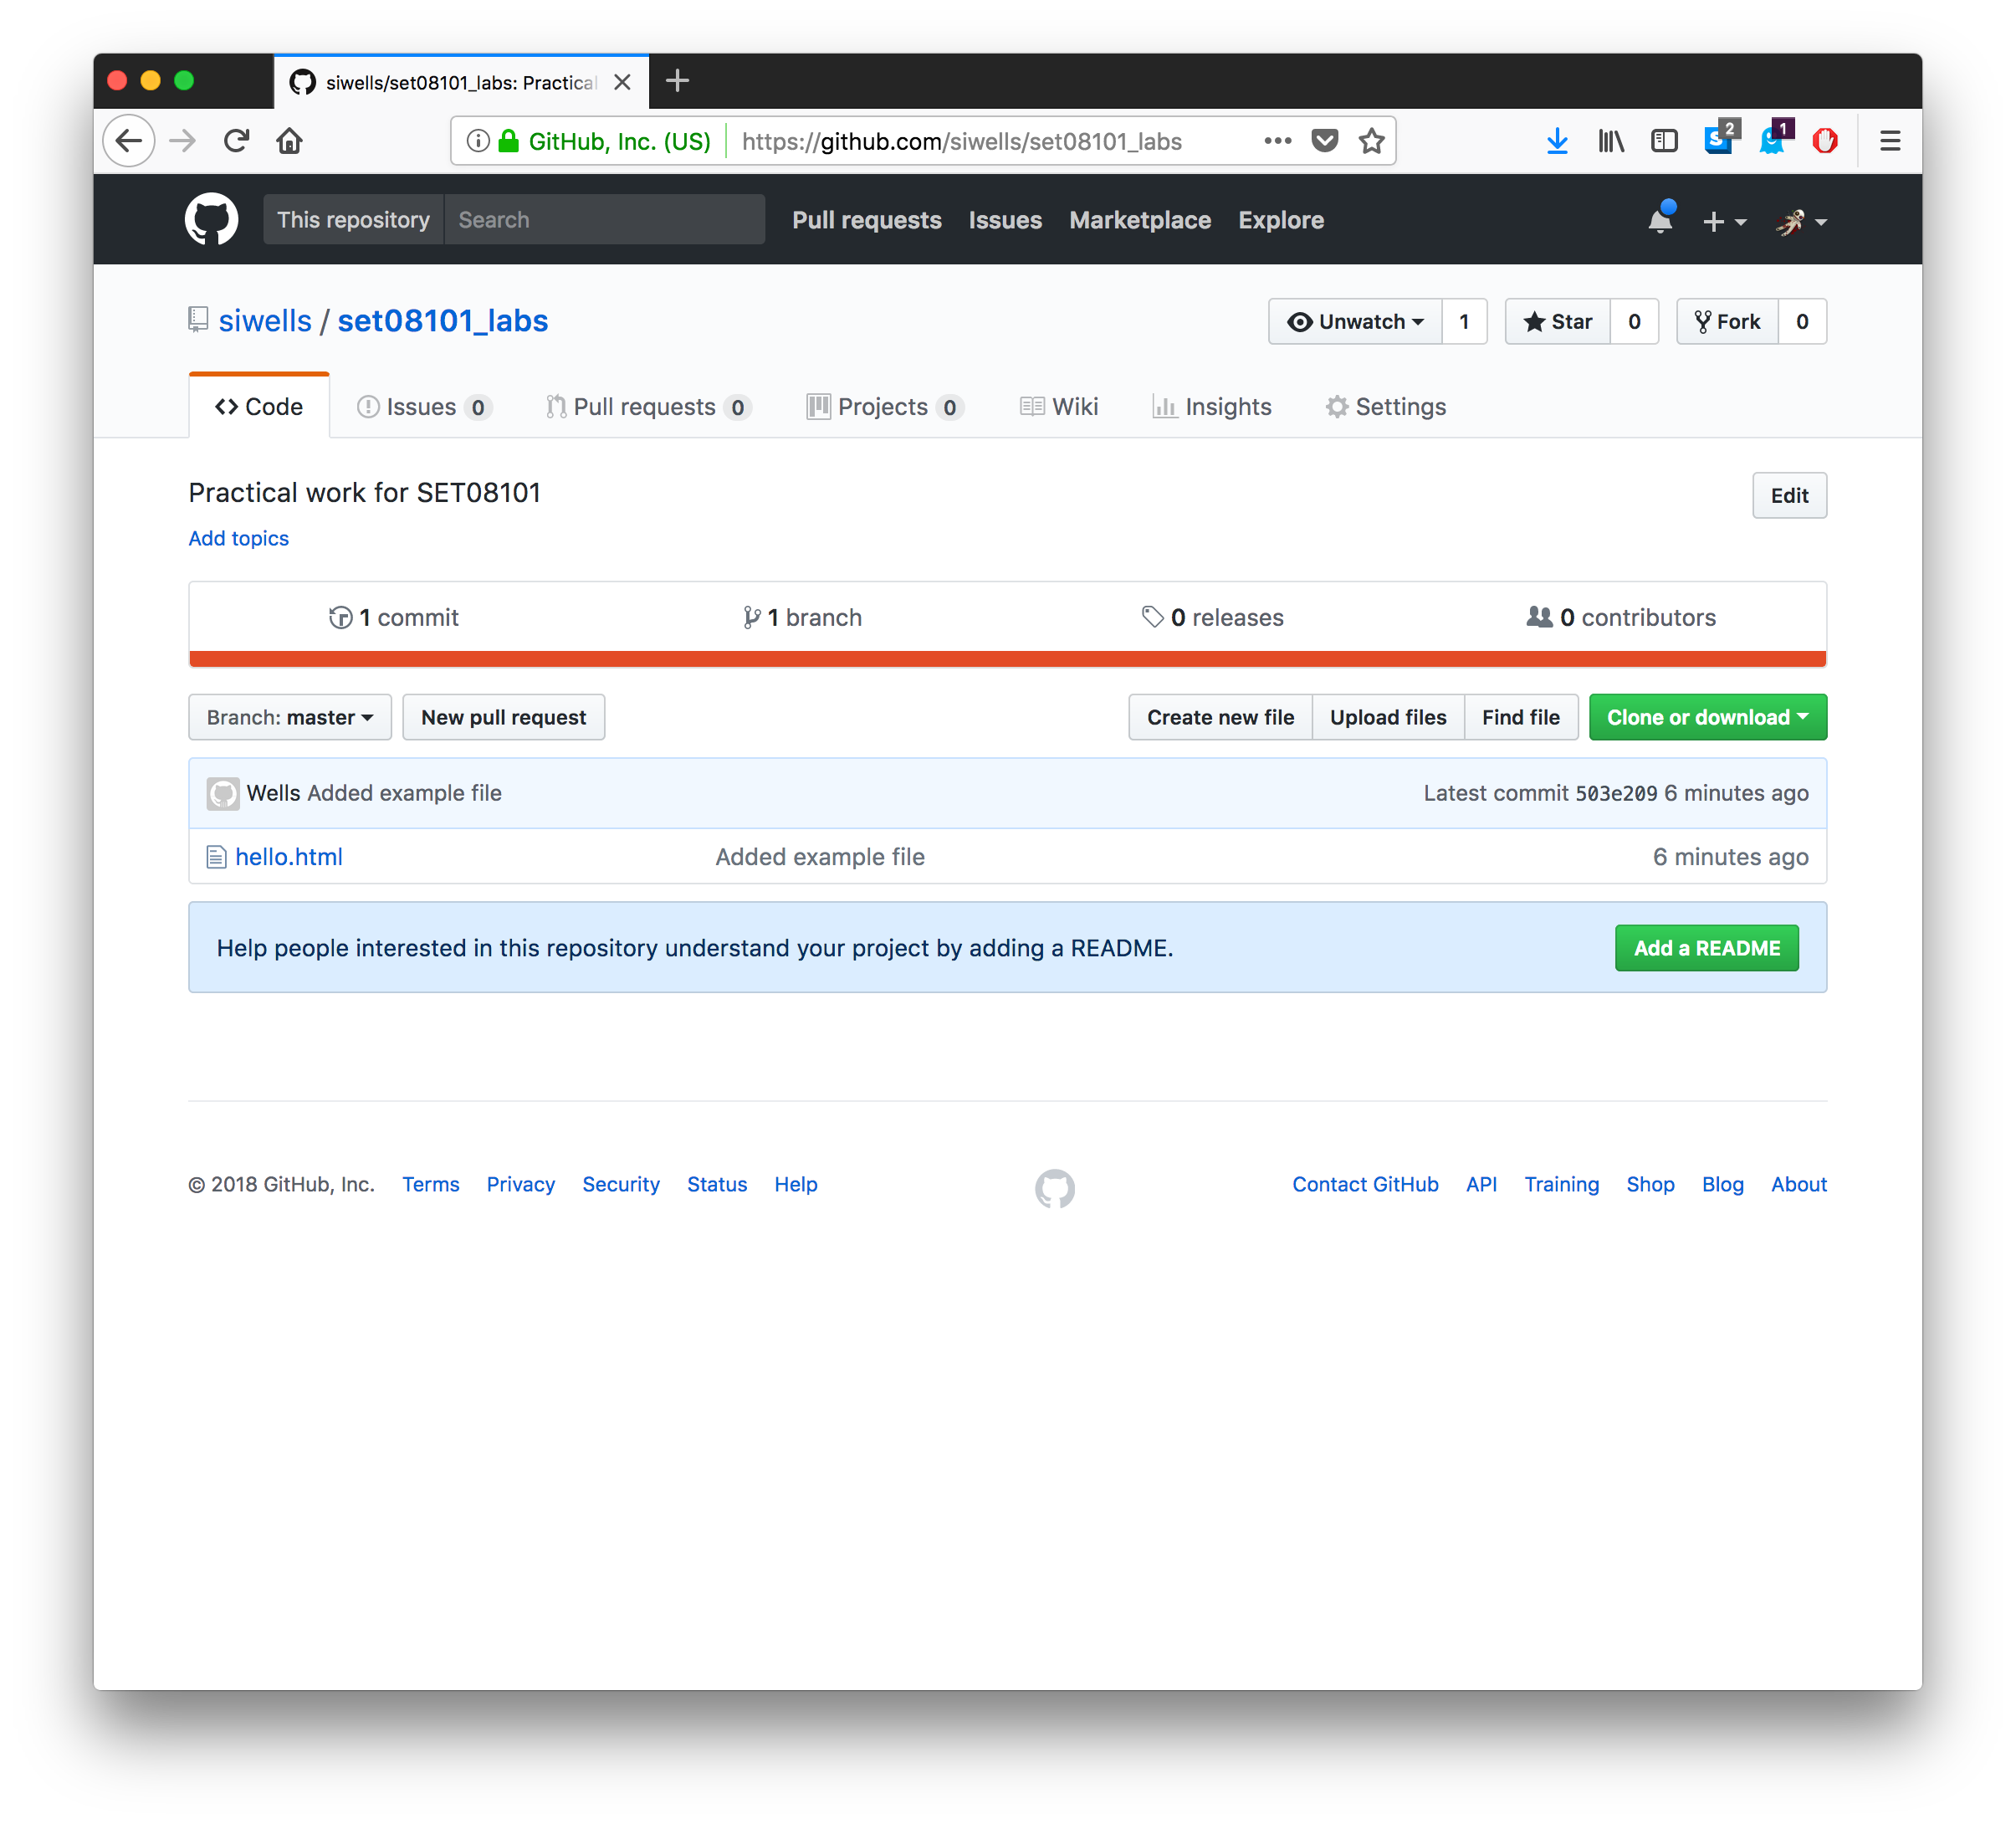
\includegraphics[width=.8\textwidth]{images/github-after-push}

\paragraph{} You can also use the Github interface to look at the files you've made changes to. This is useful sometimes to confirm that what you think is stored in GitHub actuall is, e.g.

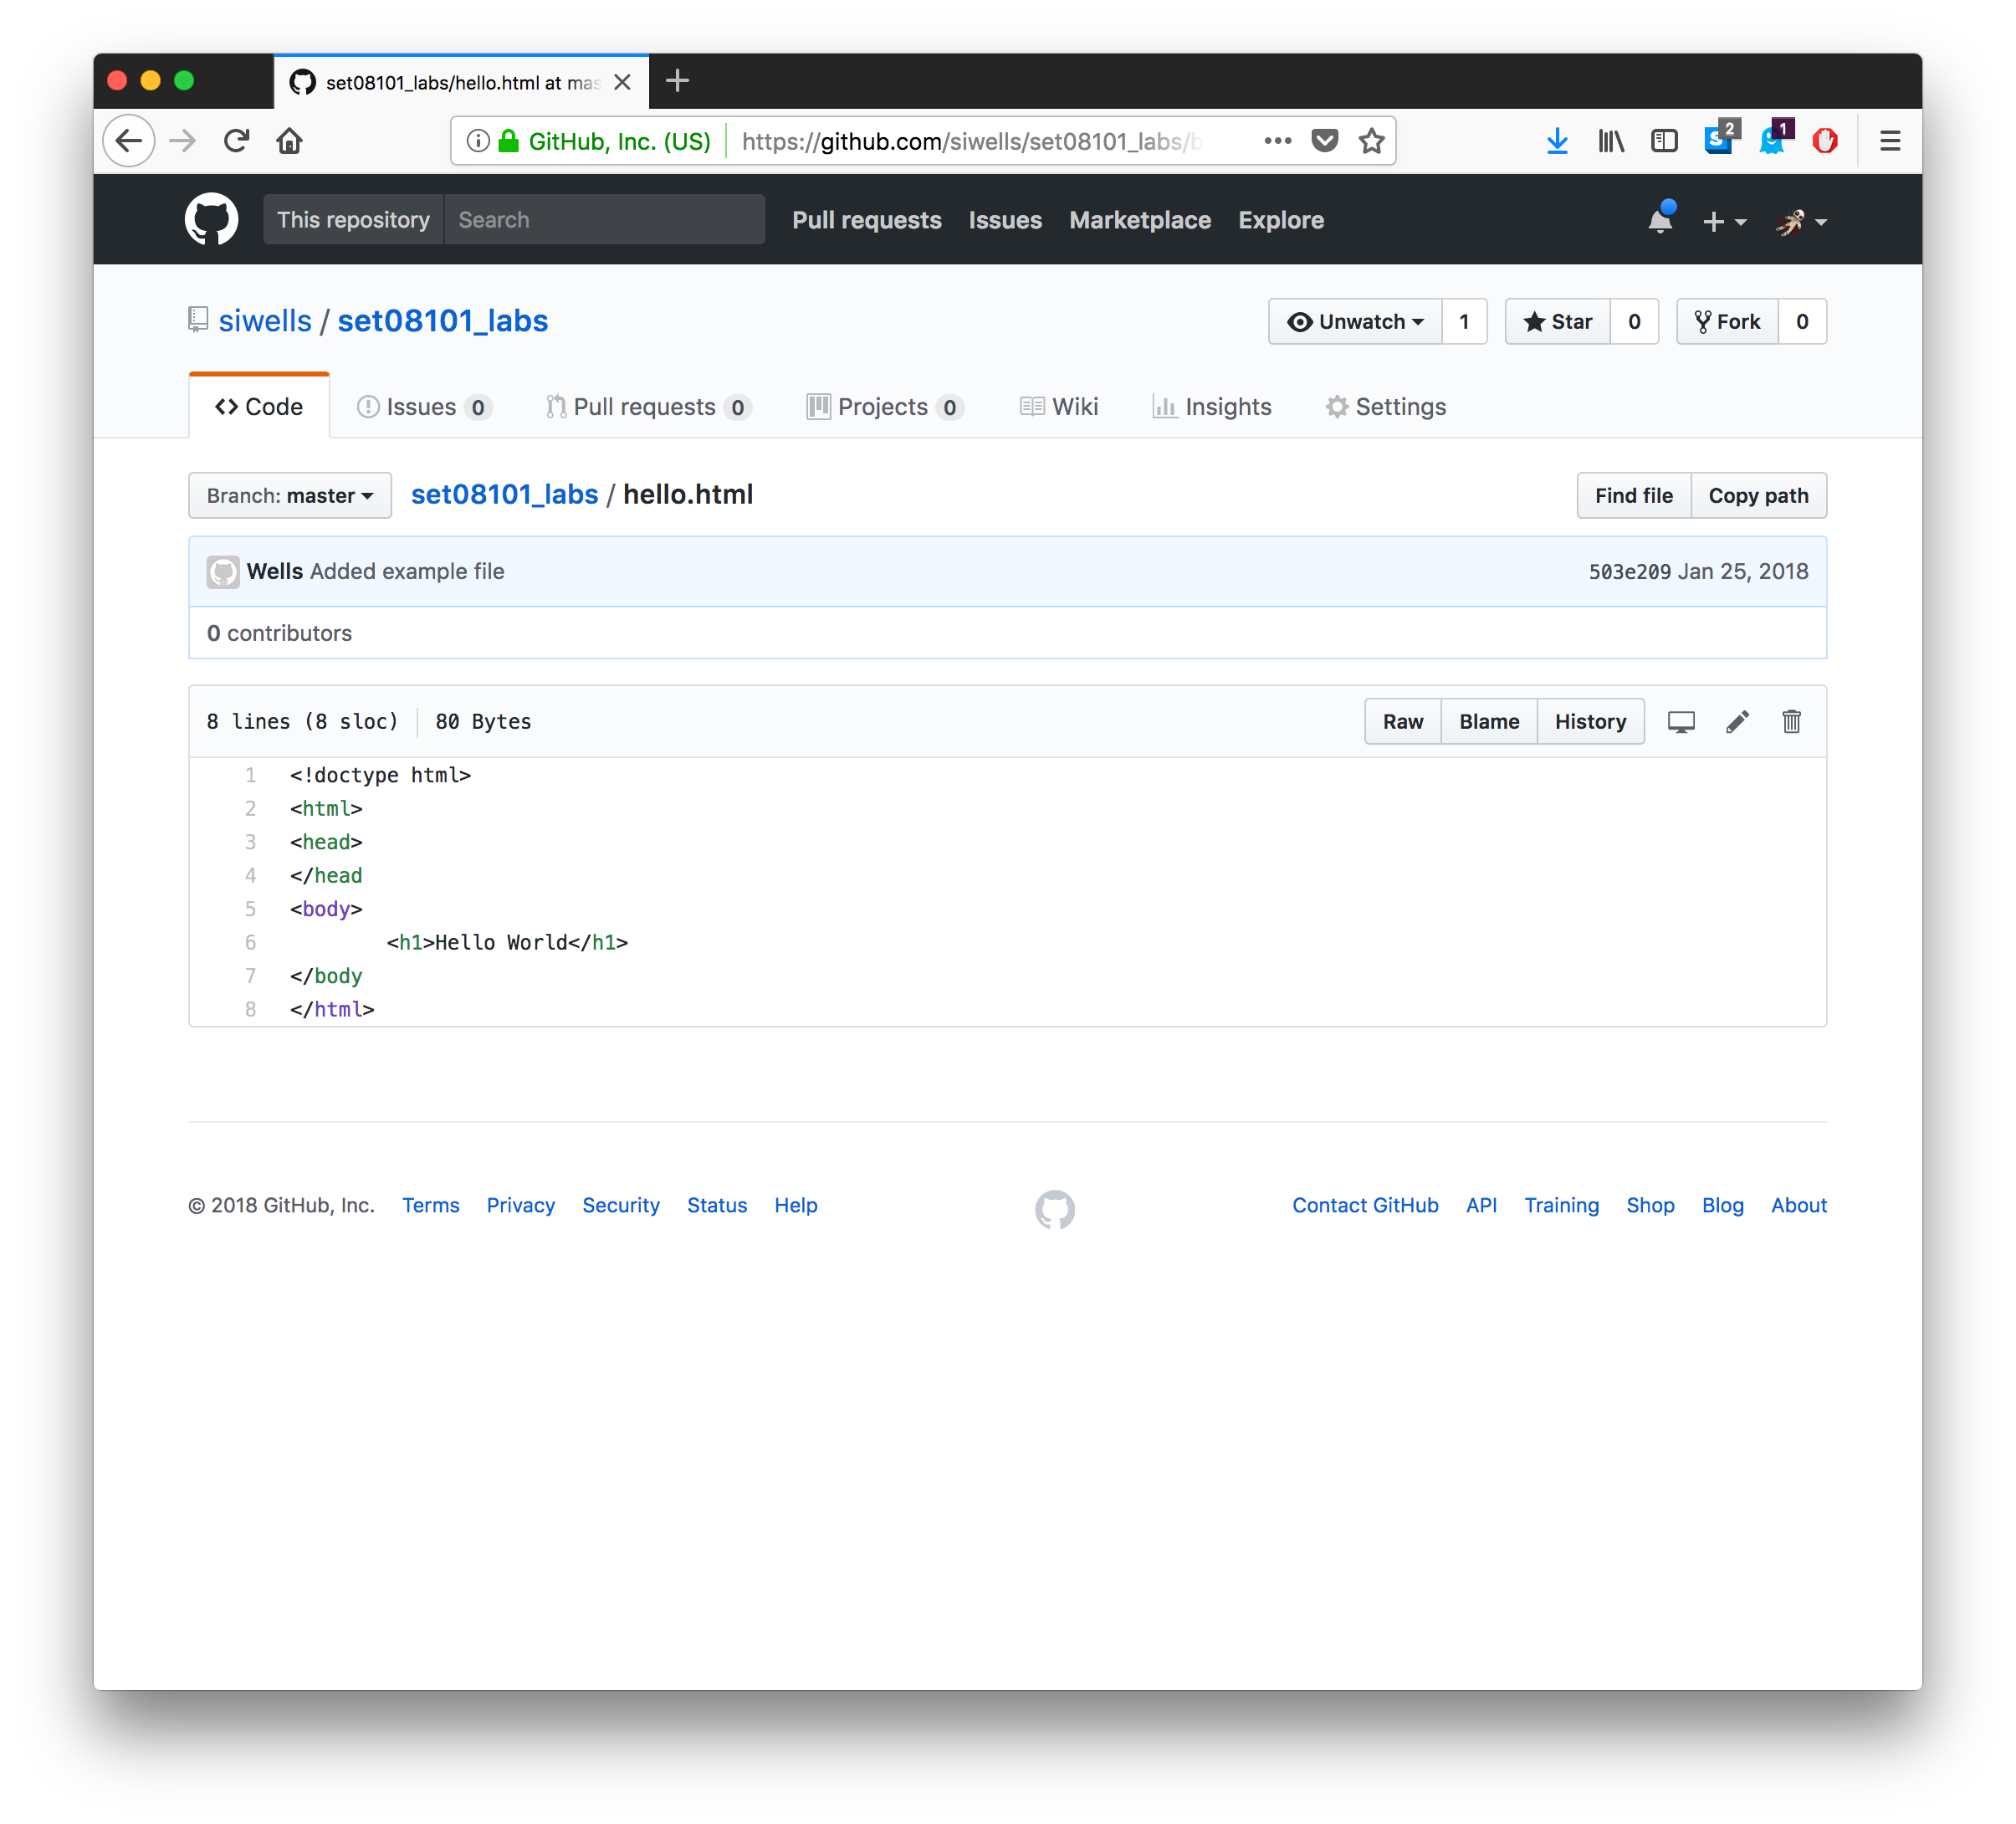
\includegraphics[width=.8\textwidth]{images/github-view-file}

\paragraph{} We need to push our work periodically so that we keep our "remote" repository up to date with any changes we've made. This gives us a useful backup of our work and also means if we want to work on our code elsewhere then all we have to do is clone our repository to the machine we are on, make changes, add and commit them, then push the changes back to GitHub.

\paragraph{} If you ever make changes to your repository from a different machine, e.g. at home, and push them to GitHub you will need to get those changes onto your lab machine. We do this with the opposite of push, we pull. Running the git pull command in your repository should fetch all new changes that are not already known locally and apply them to your code (so long as you haven't already made changes locally, in which case things get a little more complicated - but that is a story for another time [or a job for you self-directed study]).

\section{Going Further}

\paragraph{} This is only scratching the surface of Git usage.  There are also numerous interactive tutorials and resources to help you get started with Git. I'd suggest reading at least the Git parable (which explains, through example, why Git is useful) and the learn Git in 15 minutes tutorial. The important thing is to actually type in the commands and see how things work in practise rather than just reading:
\begin{enumerate}
\item The Git Parable: \url{http://tom.preston-werner.com/2009/05/19/the-git-parable.html}
\item Github's Learn Git 15 minute tutorial: \url{https://try.github.io/levels/1/challenges/1}
\item Learn Git Branching \url{http://pcottle.github.io/learnGitBranching/}
\item Git Immersion \url{http://gitimmersion.com/lab_01.html}
\end{enumerate}

%\backmatter

\bibliographystyle{plain}

\bibliography{workbook}

\end{document}

%\begin{framed}
%HELLO
%\end{framed}


%\begin{lstlisting}
%\end{lstlisting}


%\includegraphics[width=.8\textwidth]{images/}
